\chapter{Resultados y conclusiones}
%\addcontentsline{toc}{chapter}{Introduction}

La figura \ref{fig: Results} muestra las distribuciones de presión obtenidas con el \acrshort{t-mitbm} junto con las distribuciones de cálculos recientes de \acrshort{lqcd} [33]

\begin{wrapfigure}{r}{0.58\textwidth}
\centering
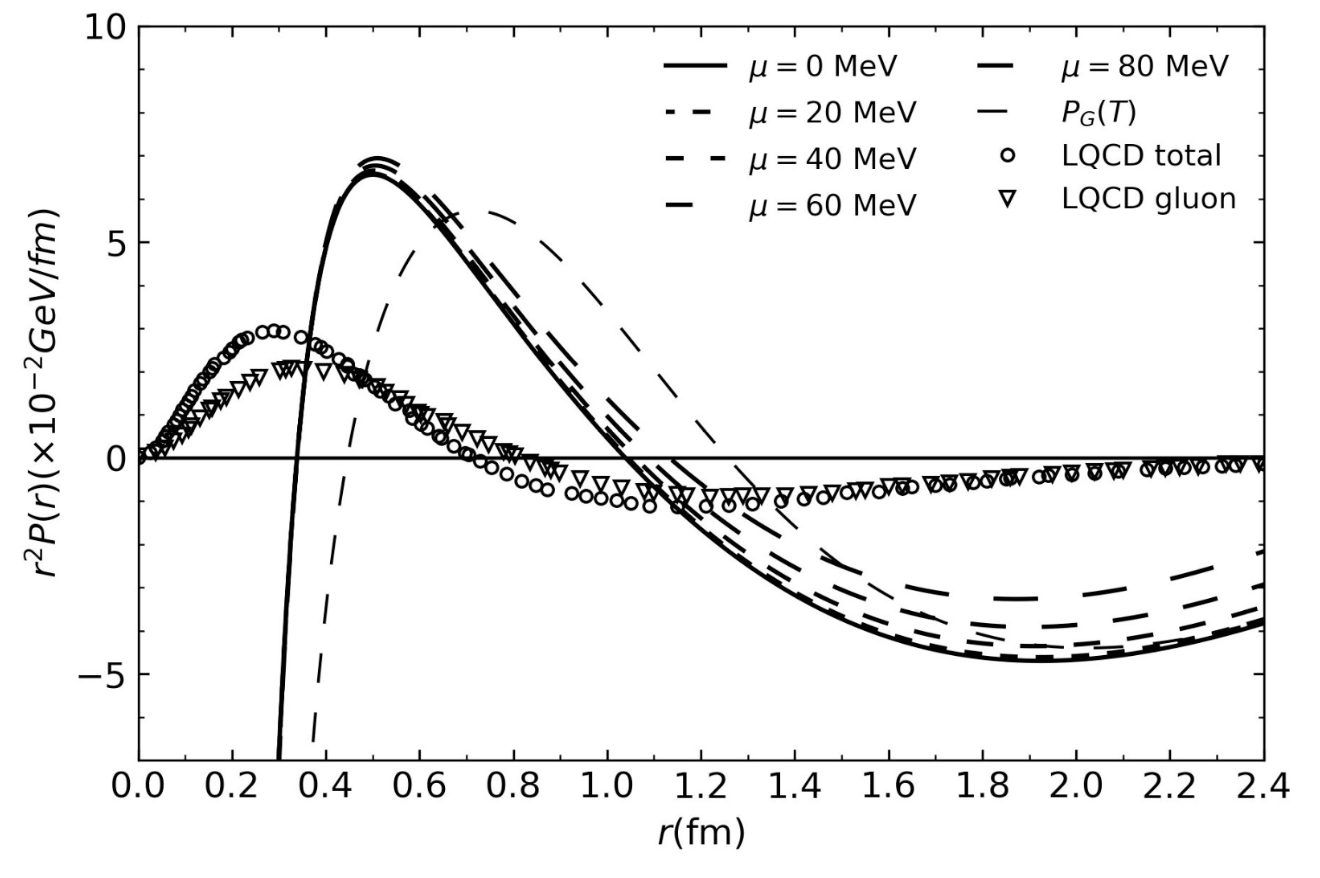
\includegraphics[width=0.58\textwidth]{./Images/MIT-BagModel.png}
\caption[MIT-Bag model]{\emph{Resultados de Lattice QCD a partir de la referencia [33], y esas obtenidas con el modelo modificado MIT bag model.}}
\label{fig: Results}
\end{wrapfigure}

$\frac{d}{dx}(x^3+x^2+1) = x (3 x + 2)$

Como se mencionó arriba, la presión de bolsa y el parámetro $q$ de Tsallis ambos representan aspectos efectivos de la interacción fuerte mediada por quarks y gluones. No tenemos un significado preciso para ellos, pero sí tenemos una relación específica entre el parámetro $q$ y la fenomenología real, como se muestra en la ecuación \eqref{eq-qasBagPress}. Creemos que la no extensividad del parámetro $q$ tiene alguna conexión con interacciones de largo alcance.

